\documentclass[/home/jesse/Analysis/FemtoAnalysis/AnalysisNotes/AnalysisNoteJBuxton.tex]{subfiles}

\renewcommand{\ResNum}{_10Res}
\renewcommand{\PrimMaxDecay}{_PrimMaxDecay4fm}

\renewcommand{\SaveNameModLamKch}{\MomRes\NonFlatBgd\ResNum\PrimMaxDecay\ResMethod\ParamFixAndShareLamKch}
\renewcommand{\SaveNameModLamKs}{\MomRes\NonFlatBgd\ResNum\PrimMaxDecay\ResMethod\ParamFixAndShareLamKs}

\begin{document}

\subsubsection{Results: \LamKs and \LamKpm: 10 Residual Correlations Included in Fit}
\label{ResultsLamK_10Res}

Figure \ref{fig:ScattParams_10Res} nicely collects and summarizes all of our extracted fit parameters for the case of 10 included residual contributors.  Figure \ref{fig:mTScalingOfRadii_10Res} presents our extracted fit radii, along with those of other systems previously analyzed by ALICE \cite{Adam:2015vja}, as a function of pair transverse mass (\mt).
Figures \ref{fig:LamK0wConjFits_10Res}, \ref{fig:LamKchPwConjFits_10Res}, and \ref{fig:LamKchMwConjFits_10Res} show the experimental correlation functions with fits, assuming 10 residual contributors, for all studied centralities for \LamKs with \ALamKs, \LamKchP with \ALamKchM, and \LamKchM with \ALamKchP, respectively.
The parameter sets extracted from the fits can be found in Tables \ref{tab:FitResultsLamK0_10Res} and \ref{tab:FitResultsLamKch_10Res}.

\begin{figure}[h]
  \centering
  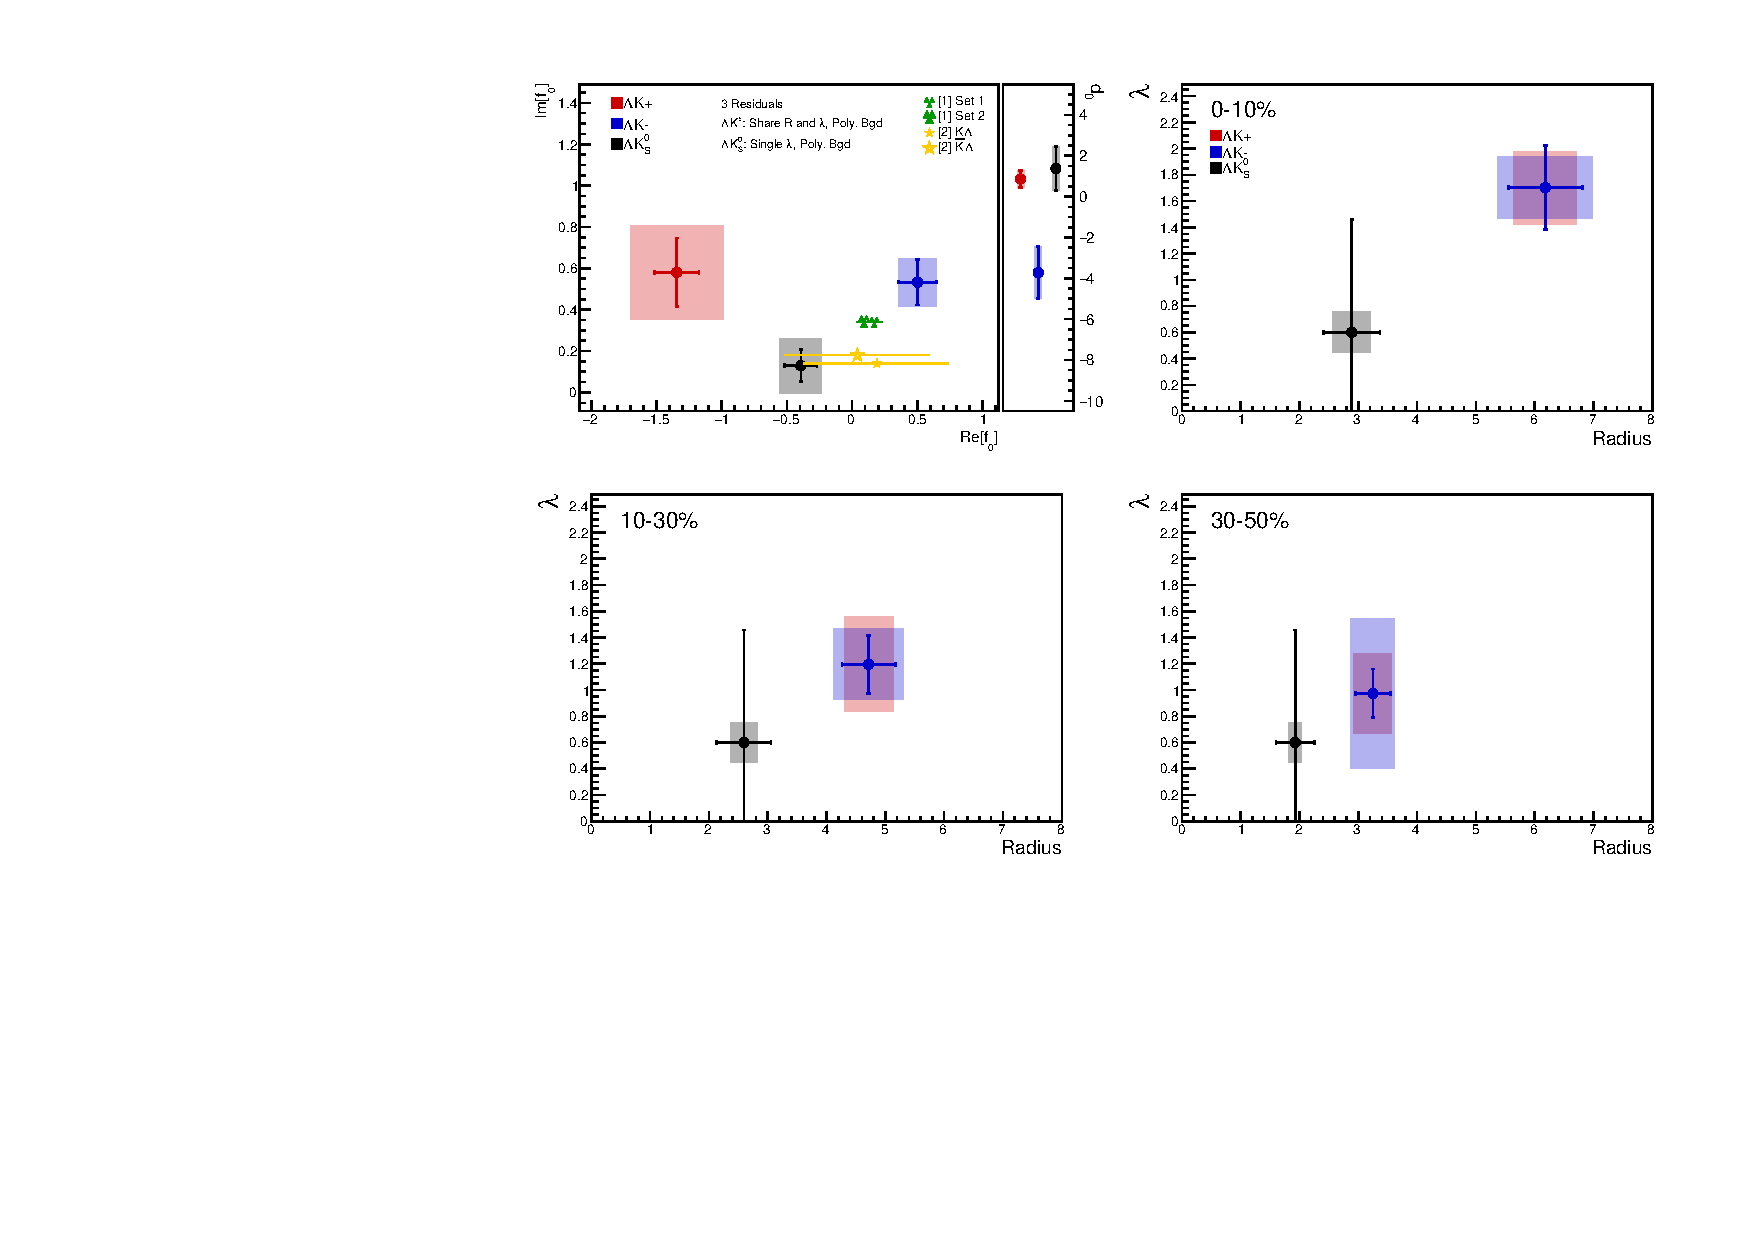
\includegraphics[width=0.80\textwidth]{7_ResultsAndDiscussion/Figures/CompareAllScattParams_Comp3An_10Res.pdf}
  \caption[Extracted Scattering Parameters: 3 Residuals in Fit]{Extracted scattering parameters for the case of 10 residual contributors for all of our $\Lambda$K systems.  [Top Left]: $\mathbb{I}f_{0}$ vs. $\mathbb{R}f_{0}$, together with d$_{0}$ to the right.  [Top Right (Bottom Left, Bottom Right)]: $\lambda$ vs. Radius for the 0-10\% (10-30\%, 30-50\%) bin.  The green \cite{Liu:2006xja} and yellow \cite{Mai:2009ce} points show theoretical predictions made using chiral perturbation theory.}
  \label{fig:ScattParams_10Res}
\end{figure}



\begin{figure}[h]
  \centering
  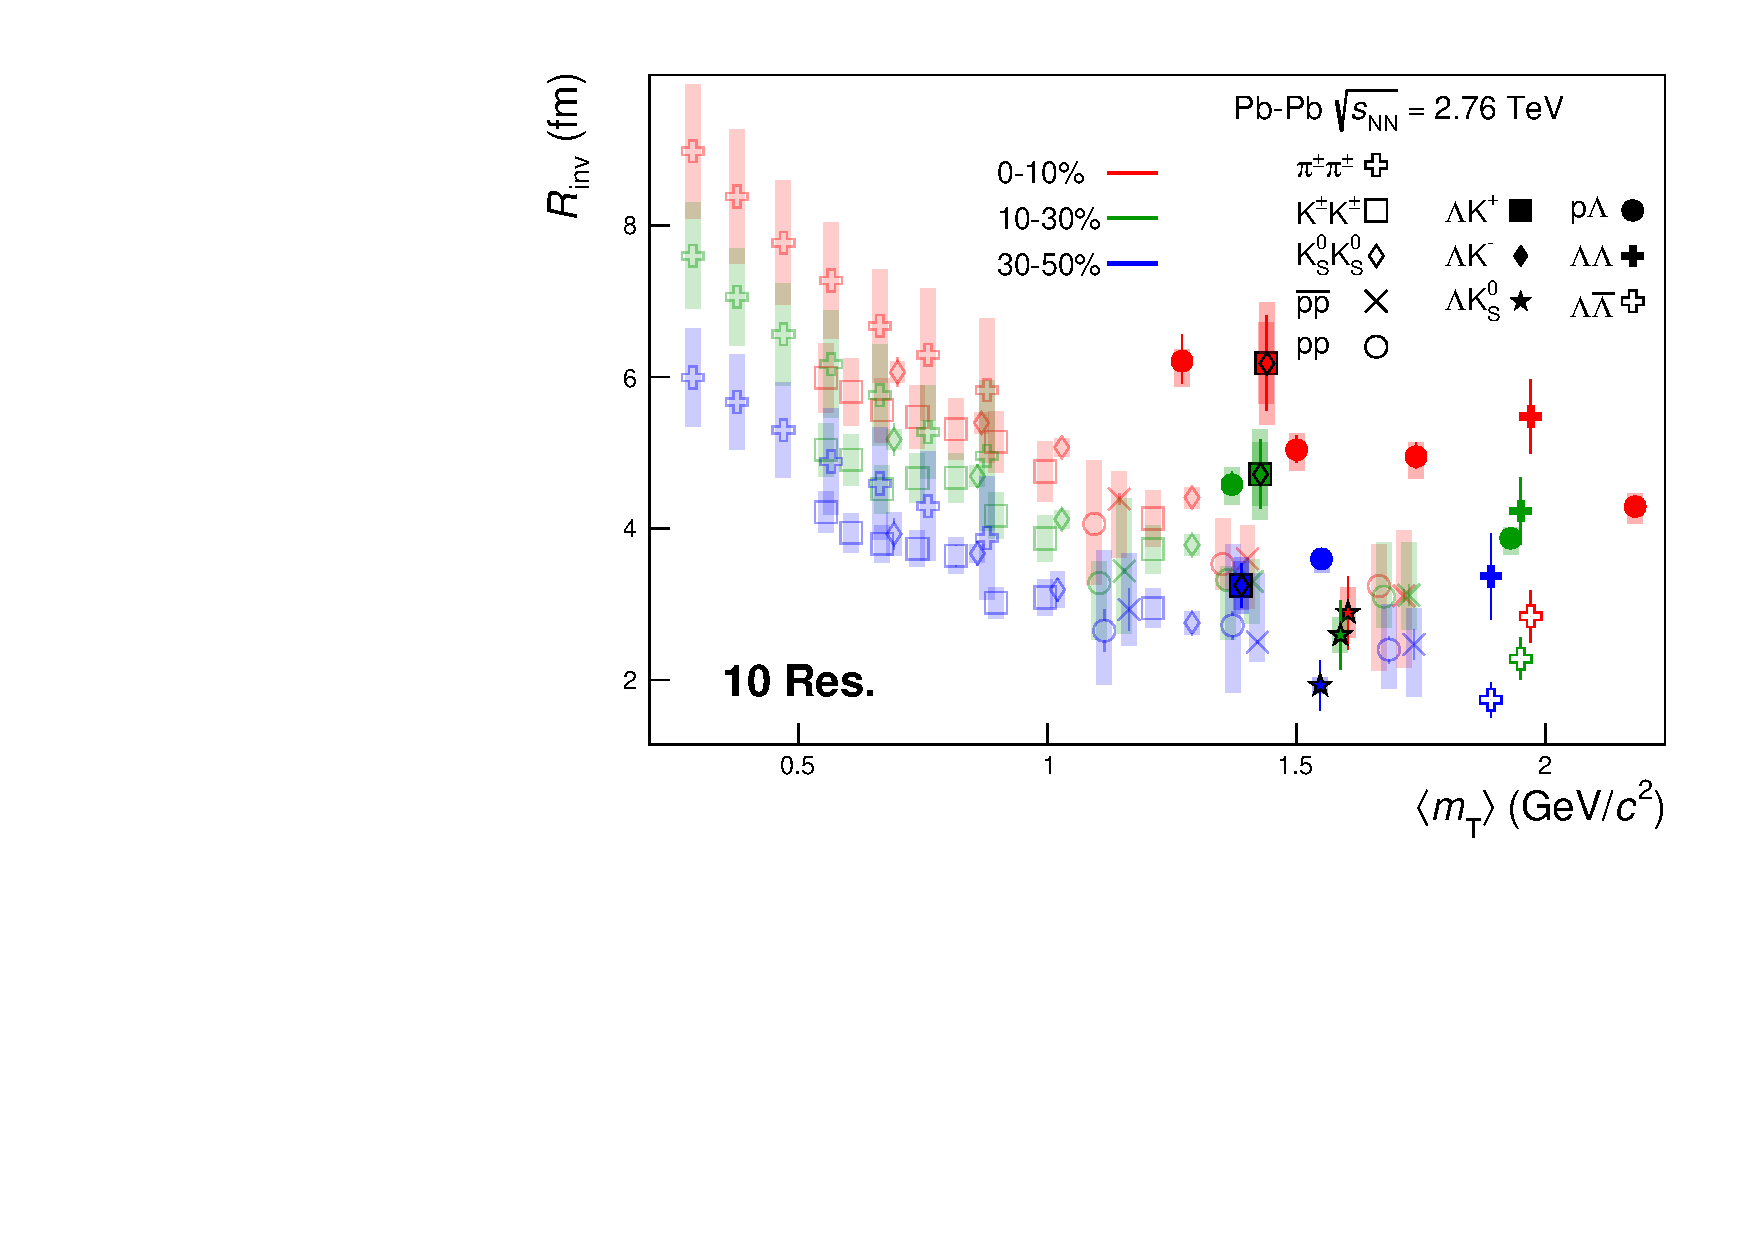
\includegraphics[width=0.50\textwidth]{7_ResultsAndDiscussion/Figures/mTscaling_MinvCalc_OutlinedPoints_OthersTransparent_wJaiAndHans_10Res.pdf}
  \caption[$m_{\mathrm{T}}$ Scaling of Radii: 10 Residuals in Fit]{10 residual correlations in $\Lambda$K fits.  Extracted fit $R_{\mathrm{inv}}$ parameters as a function of pair transverse mass ($m_{\mathrm{T}}$) for various pair systems over several centralities. The ALICE published data \cite{Adam:2015vja} is shown with transparent, open symbols.  The new $\Lambda$K results are shown with opaque, filled symbols.  In the left, the $\Lambda$K$^{+}$ (with it's conjugate pair) results are shown separately from the $\Lambda$K$^{-}$ (with it's conjugate pair) results.  In the right, all $\Lambda$K$^{\pm}$ results are averaged.}
  \label{fig:mTScalingOfRadii_10Res}
\end{figure}	

\pagestyle{empty}
\begin{landscape}

\begin{figure}[h!]
  \centering
  %%----start of first subfigure---  
  \subfloat[Signal region view ($k^{*} \lesssim 0.3$ GeV/$c$)]{
    \label{fig:LamK0wConjFits_10Res:a}
    \includegraphics[width=0.50\linewidth]{\ResultsDirBaseLamKs\SaveNameModLamKs/canKStarCfwFitsLamK0wConj_0010_1030_3050\SaveNameModLamKs.pdf}}
  %%----start of second subfigure---
  \subfloat[Wide view ($k^{*} \lesssim 1.0$ GeV/$c$)]{
    \label{fig:LamK0wConjFits_10Res:b}
    \includegraphics[width=0.50\linewidth]{\ResultsDirBaseLamKs\SaveNameModLamKs/canKStarCfwFitsLamK0wConj_0010_1030_3050UnZoomed\SaveNameModLamKs.pdf}}  
  %%----overall caption----
  \caption[$\Lambda$K$^{0}_{S}$($\bar{\Lambda}$K$^{0}_{S}$) Fits with 10 Residuals]{Fits, with 10 residual correlations included, to the $\Lambda$K$^{0}_{S}$ (left) and $\bar{\Lambda}$K$^{0}_{S}$ (right) data for the centralities 0-10\% (top), 10-30\% (middle), and 30-50\% (bottom).
 The lines represent the statistical errors, while the boxes represent the systematic errors.
 A single $\lambda$ parameter is shared amongst all.
 Each analysis has a unique normalization parameter.
 The radii are shared between analyses of like centrality, as these should have similar source sizes.
 The scattering parameters ($\mathbb{R}f_{0}$, $\mathbb{I}f_{0}$, $d_{0}$) are shared amongst all.
 The background is modeled by a (6$^{\mathrm{th}}$-)degree polynomial fit to THERMINATOR simulation.
 The black solid line represents the primary (\LamK) correlation's contribution to the fit.  
 The green line shows the fit to the non-flat background.
 The purple points show the fit after all residuals' contributions have been included, and momentum resolution and non-flat background corrections have been applied.
 The extracted fit values with uncertainties are printed.}
  \label{fig:LamK0wConjFits_10Res}
\end{figure}


\begin{figure}[h!]
  \centering
  %%----start of first subfigure---  
  \subfloat[Signal region view ($k^{*} \lesssim 0.3$ GeV/$c$)]{
    \label{fig:LamKchPwConjFits_10Res:a}
    \includegraphics[width=0.50\linewidth]{\ResultsDirBaseLamKch\SaveNameModLamKch/canKStarCfwFitsLamKchPwConj_0010_1030_3050\SaveNameModLamKch.pdf}}
  %%----start of second subfigure---
  \subfloat[Wide view ($k^{*} \lesssim 1.0$ GeV/$c$)]{
    \label{fig:LamKchPwConjFits_10Res:b}
    \includegraphics[width=0.50\linewidth]{\ResultsDirBaseLamKch\SaveNameModLamKch/canKStarCfwFitsLamKchPwConj_0010_1030_3050UnZoomed\SaveNameModLamKch.pdf}}  
  %%----overall caption----
  \caption[$\Lambda$K$^{+}$($\bar{\Lambda}$K$^{-}$) Fits with 10 Residuals]{Fits, with 10 residual correlations included, to the $\Lambda$K$^{+}$ (left) and $\bar{\Lambda}$K$^{-}$ (right) data for the centralities 0-10\% (top), 10-30\% (middle), and 30-50\% (bottom).
 The lines represent the statistical errors, while the boxes represent the systematic errors.  
 All \LamKpm analyses are fit simultaneously across all centralities (0-10\%, 10-30\%, 30-50\%).
 Scattering parameters ($\mathbb{R}f_{0}$, $\mathbb{I}f_{0}$, $d_{0}$) are shared between pair-conjugate systems (i.e. a parameter set describing the \LamKchP \& \ALamKchM system, and a separate set describing the \LamKchM \& \ALamKchP system).
 For each centrality, a radius and $\lambda$ parameters are shared between all pairs (\LamKchP, \ALamKchM, \LamKchM, \ALamKchP).
 Each analysis has a unique normalization parameter.
 The background is modeled by a (6$^{\mathrm{th}}$-)degree polynomial fit to THERMINATOR simulation.
 The black solid line represents the primary (\LamK) correlation's contribution to the fit.  
 The green line shows the fit to the non-flat background.
 The purple points show the fit after all residuals' contributions have been included, and momentum resolution and non-flat background corrections have been applied.
 The extracted fit values with uncertainties are printed.}
  \label{fig:LamKchPwConjFits_10Res}
\end{figure}



\begin{figure}[h!]
  \centering
  %%----start of first subfigure---  
  \subfloat[Signal region view ($k^{*} \lesssim 0.3$ GeV/$c$)]{
    \label{fig:LamKchMwConjFits_10Res:a}
    \includegraphics[width=0.50\linewidth]{\ResultsDirBaseLamKch\SaveNameModLamKch/canKStarCfwFitsLamKchMwConj_0010_1030_3050\SaveNameModLamKch.pdf}}
  %%----start of second subfigure---
  \subfloat[Wide view ($k^{*} \lesssim 1.0$ GeV/$c$)]{
    \label{fig:LamKchMwConjFits_10Res:b}
    \includegraphics[width=0.50\linewidth]{\ResultsDirBaseLamKch\SaveNameModLamKch/canKStarCfwFitsLamKchMwConj_0010_1030_3050UnZoomed\SaveNameModLamKch.pdf}}  
  %%----overall caption----
  \caption[$\Lambda$K$^{-}$($\bar{\Lambda}$K$^{+}$) Fits with 10 Residuals]{Fits, with 10 residual correlations included, to the $\Lambda$K$^{-}$(left) with $\bar{\Lambda}$K$^{+}$ (right) data for the centralities 0-10\% (top), 10-30\% (middle), and 30-50\% (bottom).
 The lines represent the statistical errors, while the boxes represent the systematic errors.  
 All \LamKpm analyses are fit simultaneously across all centralities (0-10\%, 10-30\%, 30-50\%).
 Scattering parameters ($\mathbb{R}f_{0}$, $\mathbb{I}f_{0}$, $d_{0}$) are shared between pair-conjugate systems (i.e. a parameter set describing the \LamKchP \& \ALamKchM system, and a separate set describing the \LamKchM \& \ALamKchP system).
 For each centrality, a radius and $\lambda$ parameters are shared between all pairs (\LamKchP, \ALamKchM, \LamKchM, \ALamKchP).
 Each analysis has a unique normalization parameter.
 The background is modeled by a (6$^{\mathrm{th}}$-)degree polynomial fit to THERMINATOR simulation.
 The black solid line represents the primary (\LamK) correlation's contribution to the fit.  
 The green line shows the fit to the non-flat background.
 The purple points show the fit after all residuals' contributions have been included, and momentum resolution and non-flat background corrections have been applied.
 The extracted fit values with uncertainties are printed.}
  \label{fig:LamKchMwConjFits_10Res}
\end{figure}



\begin{figure}[h]
  \centering
  \includegraphics[width=\textwidth]{\ResultsDirBaseLamKs\SaveNameModLamKs/Residuals\ResNum/LamK0/canKStarCfwFitsAndResidualsLamK0wConj_0010_1030_3050UnZoomed_ZoomResiduals\SaveNameModLamKs.pdf}
  \caption[\LamALamKs Fits showing 10 Residuals]{Fits, with 10 residual correlations included and shown, to the \LamKs (left) and \ALamKs (right) data for the centralities 0-10\% (top), 10-30\% (middle), and 30-50\% (bottom).  The ten parent pairs used for the residual correction to the \LamKs (\ALamKs) fit are $\Sigma^{0}$\Ks, $\Xi^{0}$\Ks, $\Xi^{-}$\Ks, $\Sigma^{*(+,-,0)}$\Ks, $\Lambda$K$^{*0}$, $\Sigma^{0}$K$^{*0}$, $\Xi^{0}$K$^{*0}$, and $\Xi^{-}$K$^{*0}$ ($\bar{\Sigma}^{0}$\Ks, $\bar{\Xi}^{0}$\Ks, $\bar{\Xi}^{+}$\Ks, $\bar{\Sigma}^{*(+,-,0)}$\Ks, $\bar{\Lambda}\bar{\mathrm{K}}^{*0}$, $\bar{\Sigma}^{0}\bar{\mathrm{K}}^{*0}$, $\bar{\Xi}^{0}\bar{\mathrm{K}}^{*0}$, and $\bar{\Xi}^{+}\bar{\mathrm{K}}^{*0}$).}
  \label{fig:LamK0wConjFitsAndResiduals_10Res}
\end{figure}


\begin{figure}[h!]
  \centering
  %%----start of first subfigure---  
  \subfloat[\LamKchPALamKchM fits with residual contributions shown for the centralities 0-10\% (top), 10-30\% (middle), and 30-50\% (bottom)]{
    \label{fig:LamKchwConjFitsAndResiduals_10Res:a}
    \includegraphics[width=0.50\linewidth]{\ResultsDirBaseLamKch\SaveNameModLamKch/Residuals\ResNum/LamKchP/canKStarCfwFitsAndResidualsLamKchPwConj_0010_1030_3050UnZoomed_ZoomResiduals\SaveNameModLamKch.pdf}}
  %%----start of second subfigure---
  \subfloat[\LamKchMALamKchP fits with residual contributions shown for the centralities 0-10\% (top), 10-30\% (middle), and 30-50\% (bottom)]{
    \label{fig:LamKchwConjFitsAndResiduals_10Res:b}
    \includegraphics[width=0.50\linewidth]{\ResultsDirBaseLamKch\SaveNameModLamKch/Residuals\ResNum/LamKchM/canKStarCfwFitsAndResidualsLamKchMwConj_0010_1030_3050UnZoomed_ZoomResiduals\SaveNameModLamKch.pdf}}  
  %%----overall caption----
  \caption[\LamKchPALamKchM and \LamKchMALamKchP Fits with 10 Residuals]{Fits, with 10 residual correlations included and shown, to the \LamKchP \& \ALamKchM (left) and \LamKchM \& \ALamKchP (right) data for the centralities 0-10\% (top), 10-30\% (middle), and 30-50\% (bottom).  The ten parent pairs used for the residual correction to the \LamKchP (\ALamKchM) fit are $\Sigma^{0}$\KchP, $\Xi^{0}$\KchP, $\Xi^{-}$\KchP, $\Sigma^{*(+,-,0)}$\KchP, $\Lambda$K$^{*0}$, $\Sigma^{0}$K$^{*0}$, $\Xi^{0}$K$^{*0}$, and $\Xi^{-}$K$^{*0}$ ($\bar{\Sigma}^{0}$\KchM, $\bar{\Xi}^{0}$\KchM, $\bar{\Xi}^{+}$\KchM, $\bar{\Sigma}^{*(+,-,0)}$\KchM, $\bar{\Lambda}\bar{\mathrm{K}}^{*0}$, $\bar{\Sigma}^{0}\bar{\mathrm{K}}^{*0}$, $\bar{\Xi}^{0}\bar{\mathrm{K}}^{*0}$, and $\bar{\Xi}^{+}\bar{\mathrm{K}}^{*0}$).}
  \label{fig:LamKchwConjFitsAndResiduals_10Res}
\end{figure}



\end{landscape}
\pagestyle{plain}


%%%%%%%%%%%%%%%%%%%%%%%%%%%%%%%%%%%%%%%%     TABLES!!!!!     %%%%%%%%%%%%%%%%%%%%%%%%%%%%%%%%%%%%%%%%
\subfile{7_ResultsAndDiscussion/7.1_ResultsLamK/7.1.3_ResultsLamK_10Res/7.1.3_ResultsTables_10Res/7.1.3_ResultsTables_10Res.tex}
%%%%%%%%%%%%%%%%%%%%%%%%%%%%%%%%%%%%%%%%%%%%%%%%%%%%%%%%%%%%%%%%%%%%%%%%%%%%%%%%%%%%%%%%%%%%%%%%%%%%%


\clearpage

\end{document}